%\chapter*{Appendix}
\appendix
\begin{landscape}
% c2d vs i7 shsp !!
\begin{figure}[H]
    \subfloat[Core 2 Duo search time] {
        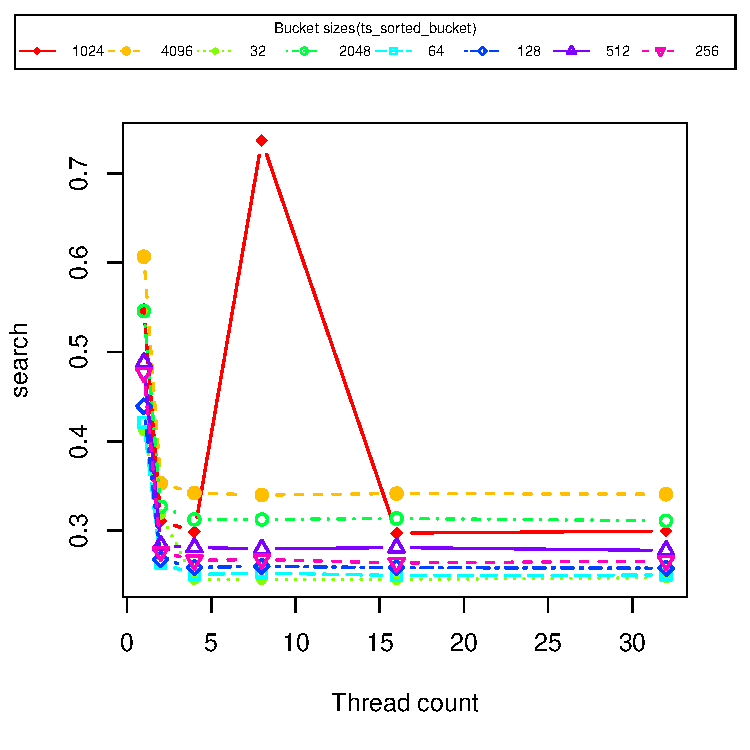
\includegraphics[width=1.0\textwidth]{plots/c2d/plot_1_ts_sorted_bucketsearch}
    }
    \subfloat[Core i7 search time] {
        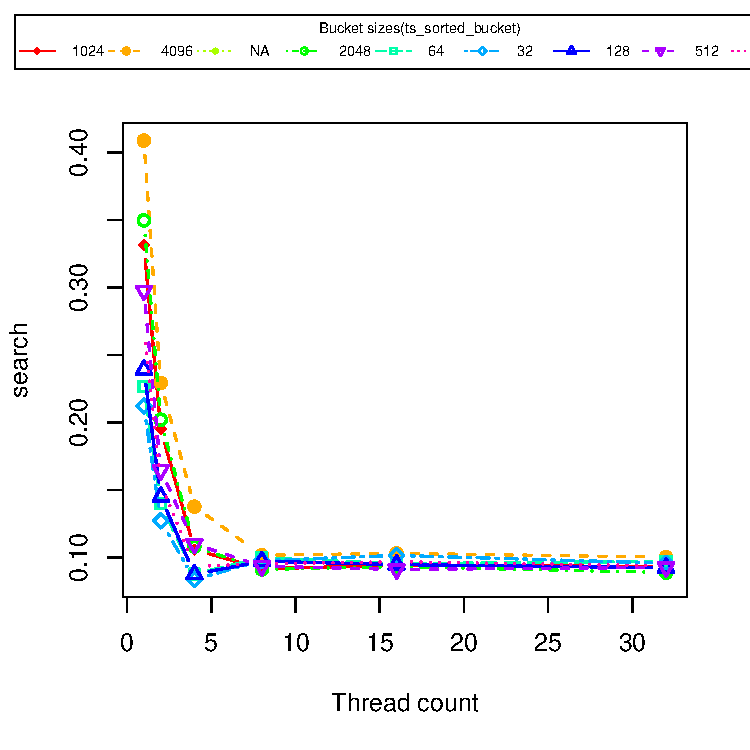
\includegraphics[width=1.0\textwidth]{plots/i7/plot_1_ts_sorted_bucketsearch}
    }
    \label{fig:ts_shsp}
    \caption{Shakespeare tests: Multithreaded scaling of the unsorted dynamic
    array bucket with varying sizes on the i7 machine (quad-core) and the c2d
    machine (dual-core).}
\end{figure}
% i7 30m !!
\begin{figure}[H]
    \subfloat[Sorted bucket insert on the i7.] {
        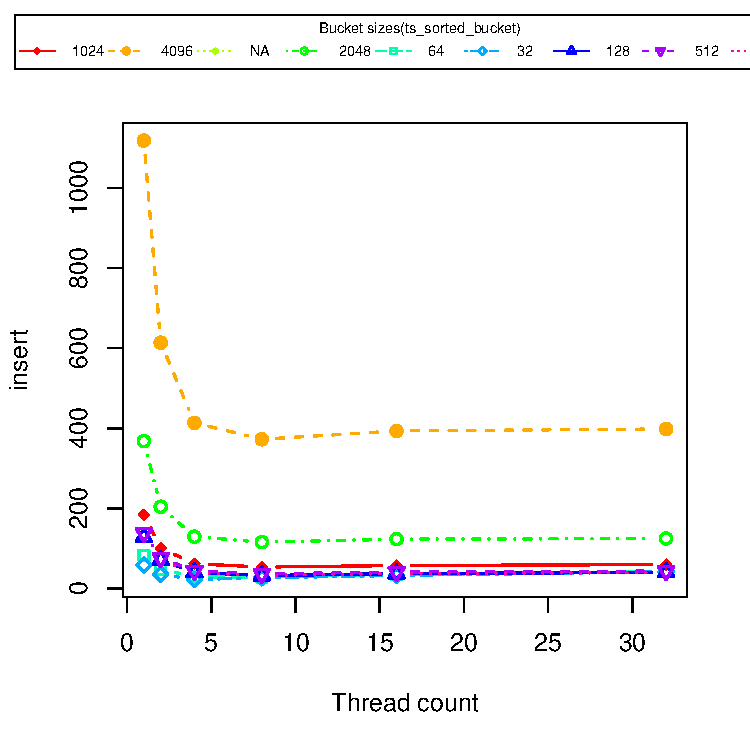
\includegraphics[width=1.0\textwidth]{plots/i7/plot_0_ts_sorted_bucketinsert}
    }
    \subfloat[Unsorted bucket insert on the i7. The same tendencies were found
        with {\keyword map} and binary tree buckets.] {
        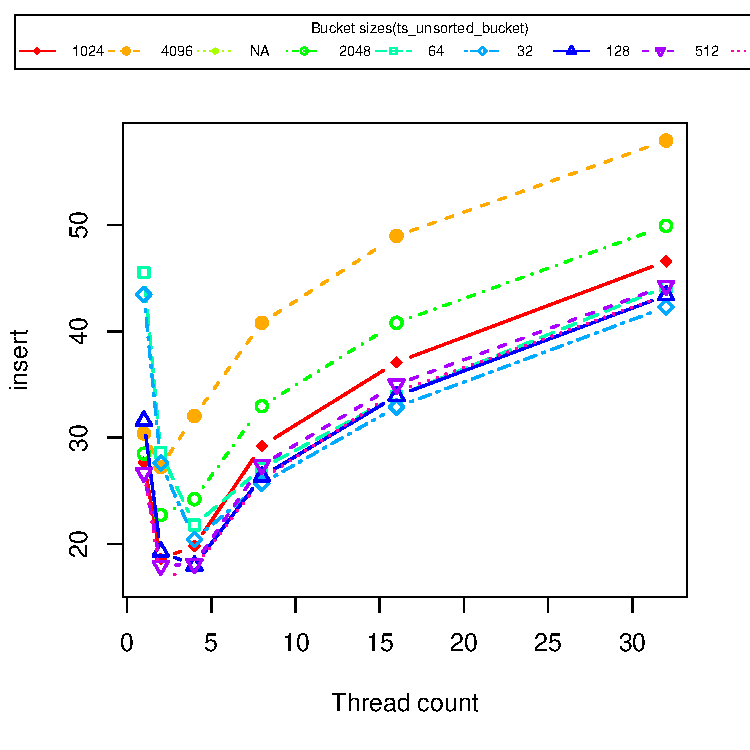
\includegraphics[width=1.0\textwidth]{plots/i7/plot_0_ts_unsorted_bucketinsert}
    }
    \label{fig:ts_i7_30m}
    \caption{30M i7: Multithreaded scaling of the sorted dynamic array bucket with varying sizes on the
    i7 machine (quad-core). Testing done with the 30M dataset.}
\end{figure}
\begin{figure}[H]
    \subfloat[Sorted bucket insert on the i7. The same tendencies were found with the binary tree.] {
        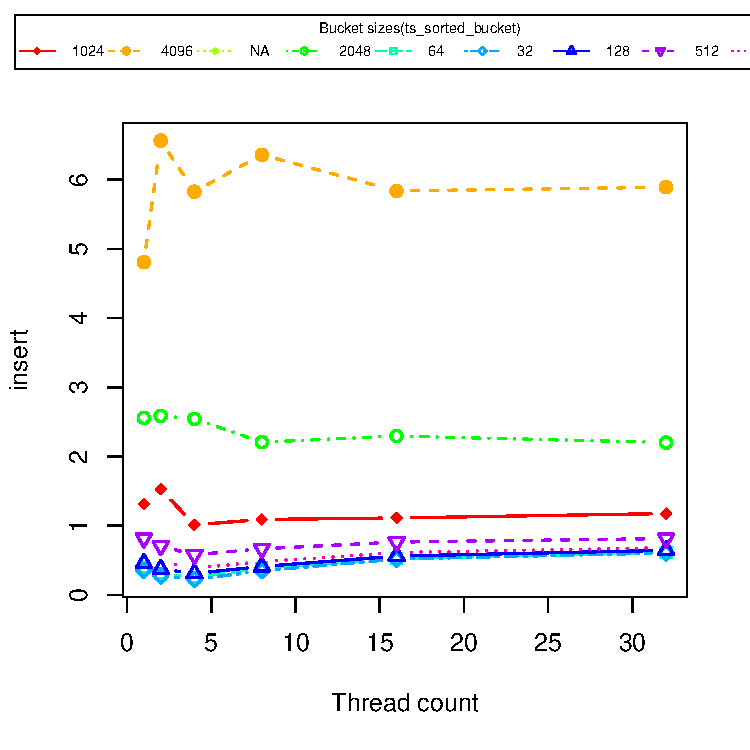
\includegraphics[width=1.0\textwidth]{plots/i7/plot_1_ts_sorted_bucketinsert}
    }
    \subfloat[Unsorted bucket insert on the i7. The same tendencies were found with  {\keyword map}.] {
        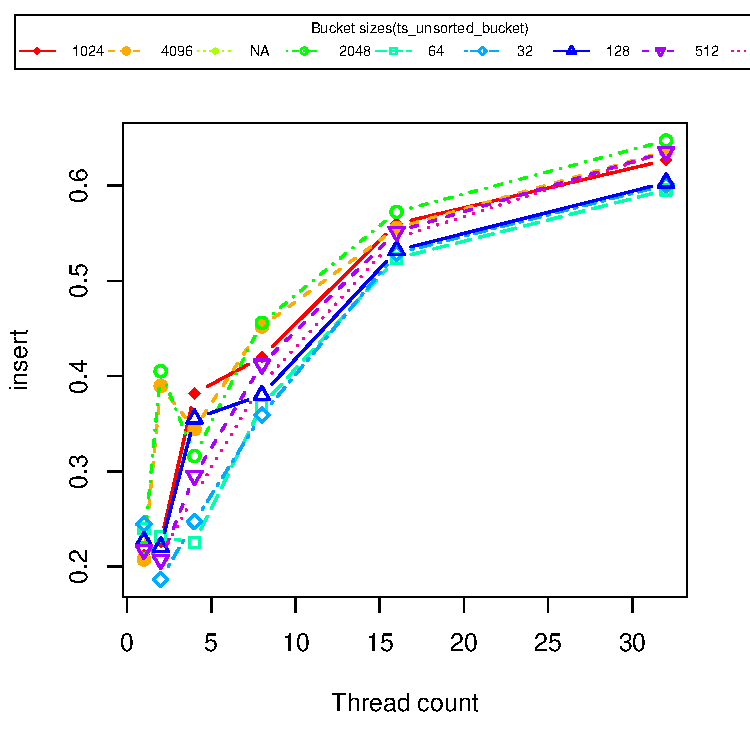
\includegraphics[width=1.0\textwidth]{plots/i7/plot_1_ts_unsorted_bucketinsert}
    }
    \label{fig:ts_i7_nsgrp}
    \caption{Newsgroups i7: Multithreaded scaling of the array bucket with varying sizes on the
    i7 machine (quad-core). Testing done with the Newsgroups dataset.}
\end{figure}
\end{landscape}
